\documentclass[letterpaper]{ut-thesis}%{report}
\usepackage{graphicx}

\newcommand{\captionpart}[1]{\textbf{#1}}

\begin{document}

\graphicspath{{figs-techreport/}}

\begin{figure}[htp]
\begin{center}
\setlength{\fboxsep}{0.5pt}
\setlength{\fboxrule}{0.25pt}
\framebox{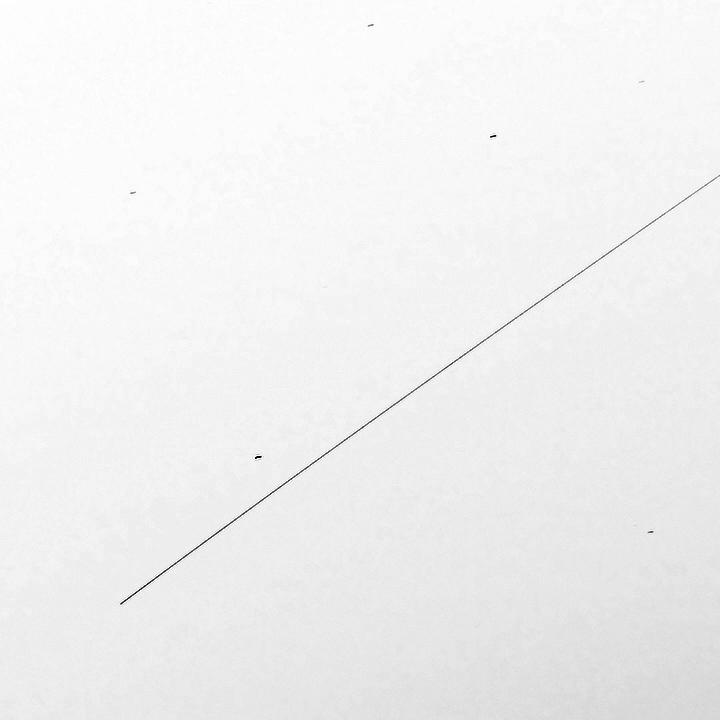
\includegraphics[width=0.55\textwidth]{iss-inv}}%
\\
\framebox{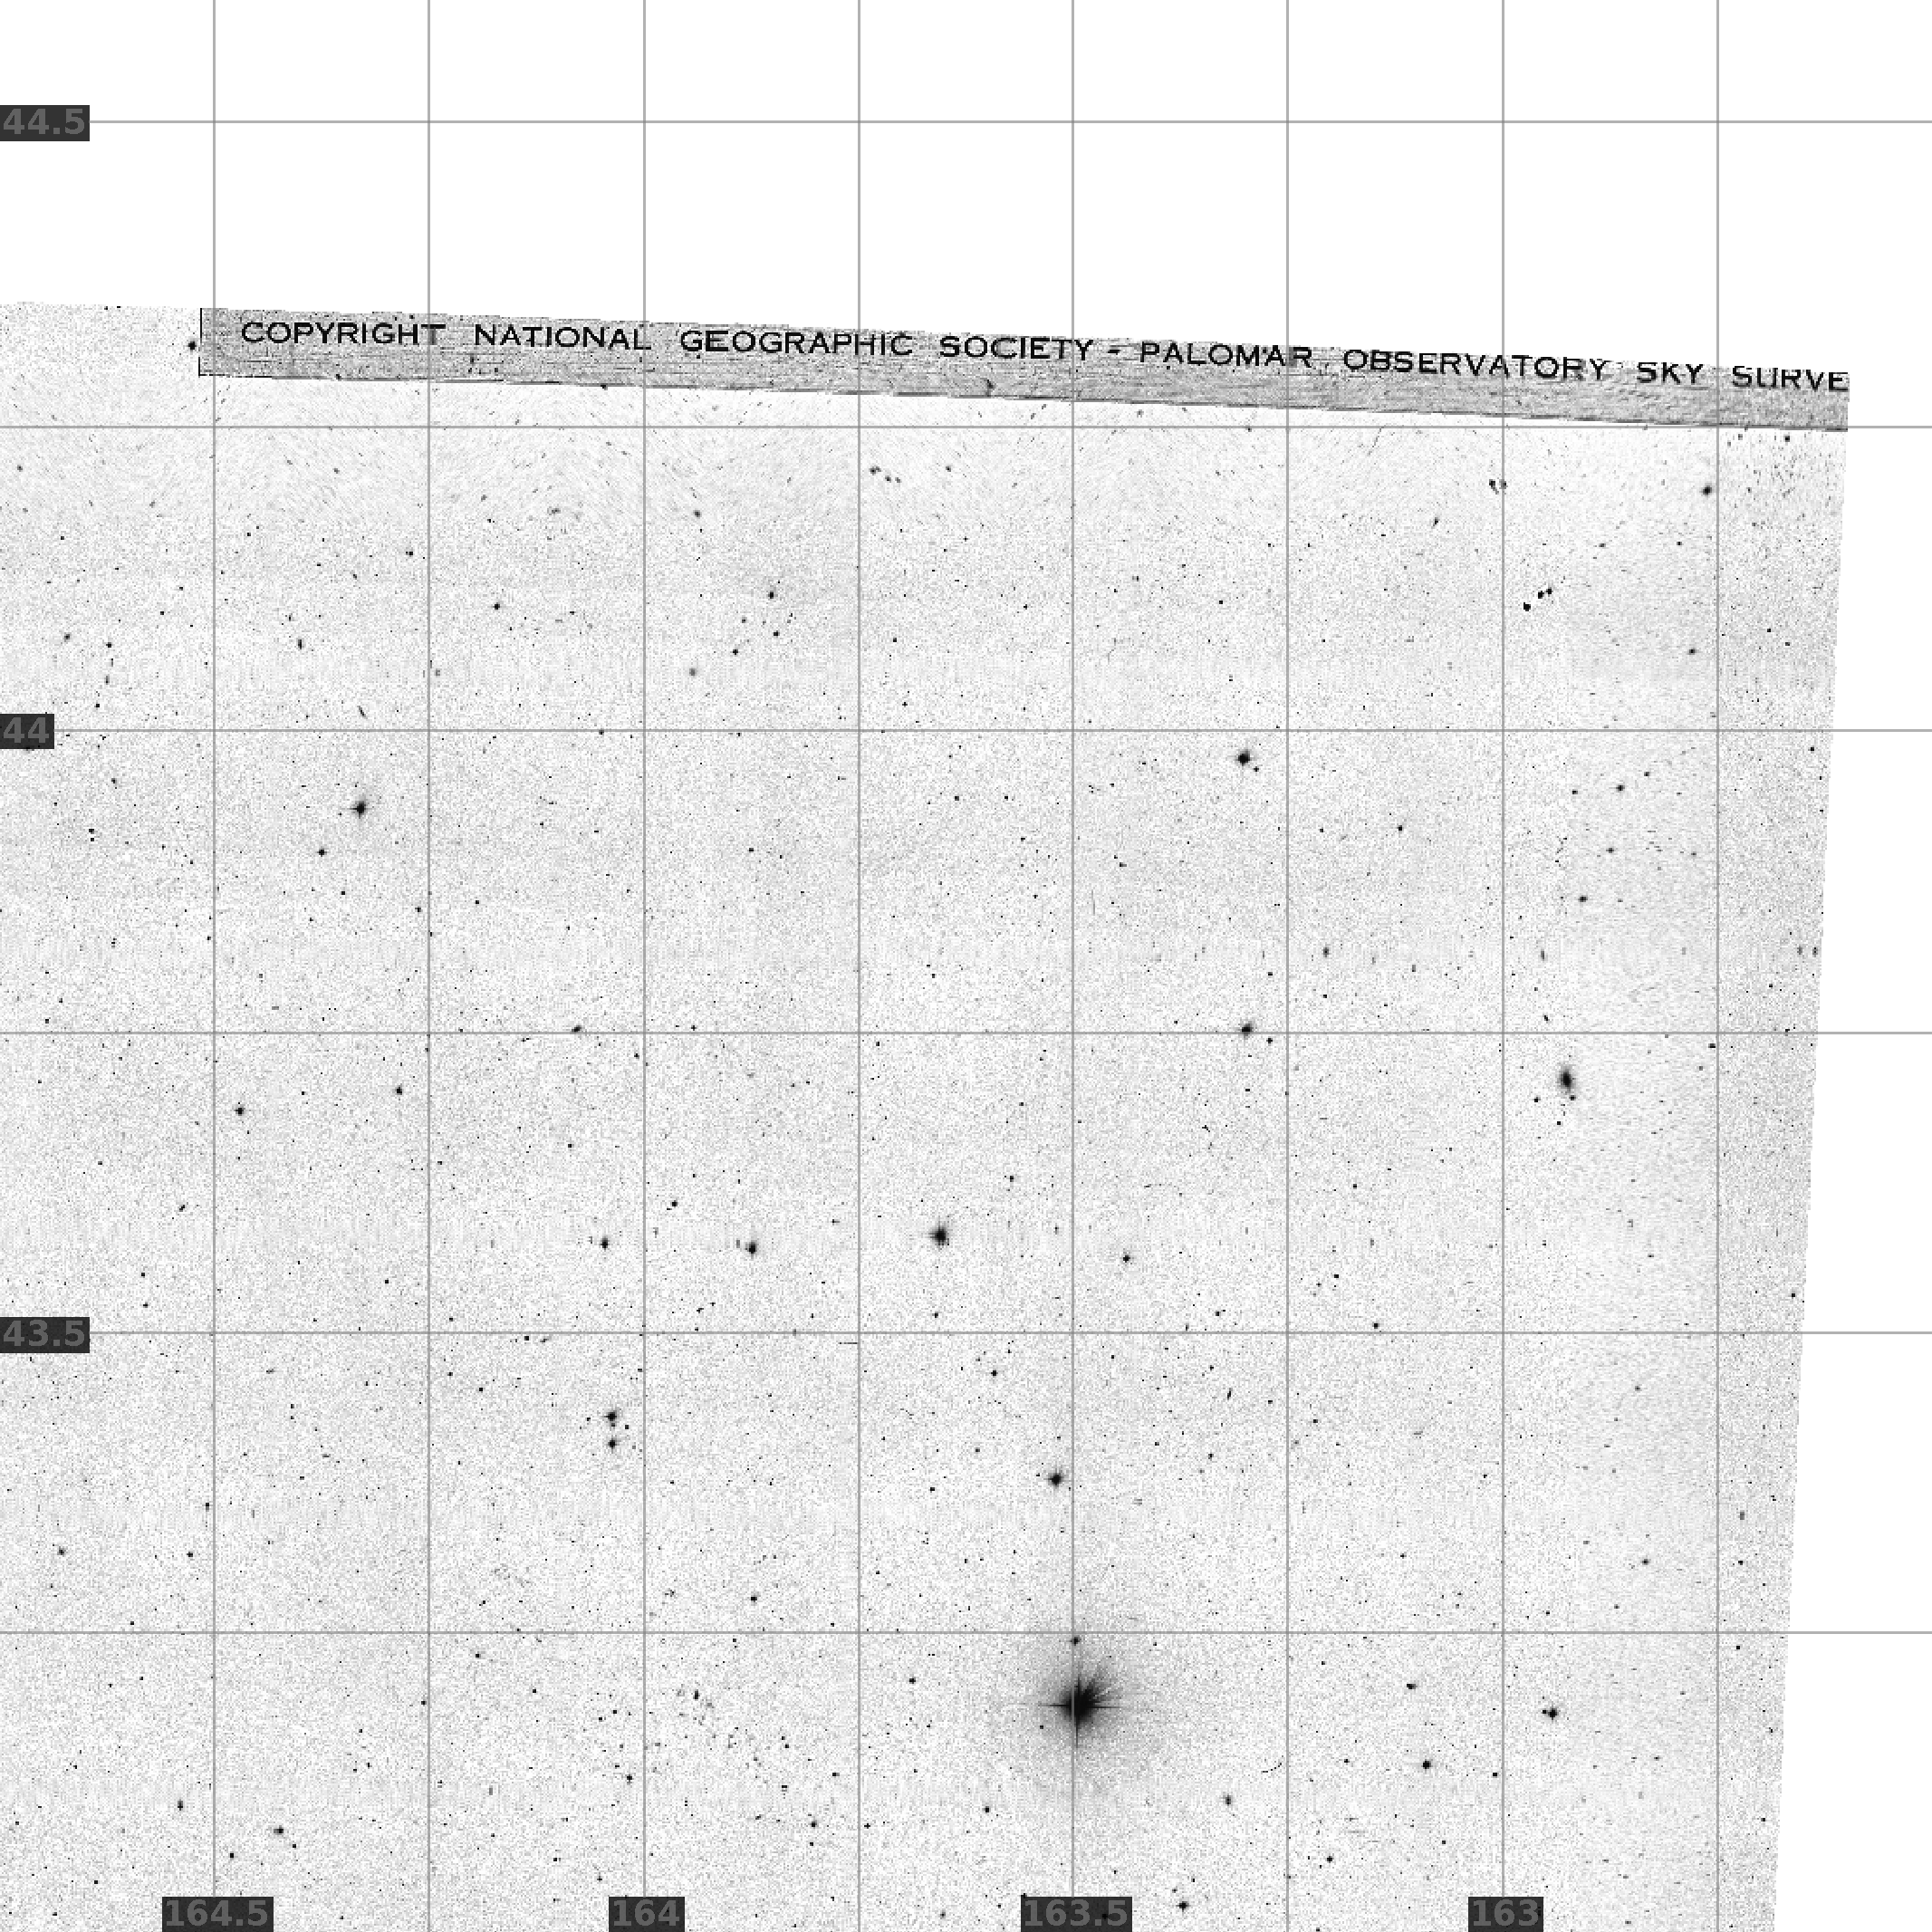
\includegraphics[width=0.55\textwidth]{usnob-iss}}%
\end{center}
\caption{A false-positive match.  \captionpart{Top:} The input image
contains a linear feature: the International Space Station streaked
across the image.  Image credit: copyright Massimo Matassi.
\captionpart{Bottom:} The USNO-B scanned photographic plate has
writing on the corner.  Image credit: copyright Palomar Observatory,
National Geographic Society, and California Institute of Technology;
courtesy of USNO Image and Catalogue Archive.
\label{fig:falseposA}}
\end{figure}

\begin{figure}[htp]
\begin{center}
\setlength{\fboxsep}{0.5pt}
\setlength{\fboxrule}{0.25pt}
\framebox{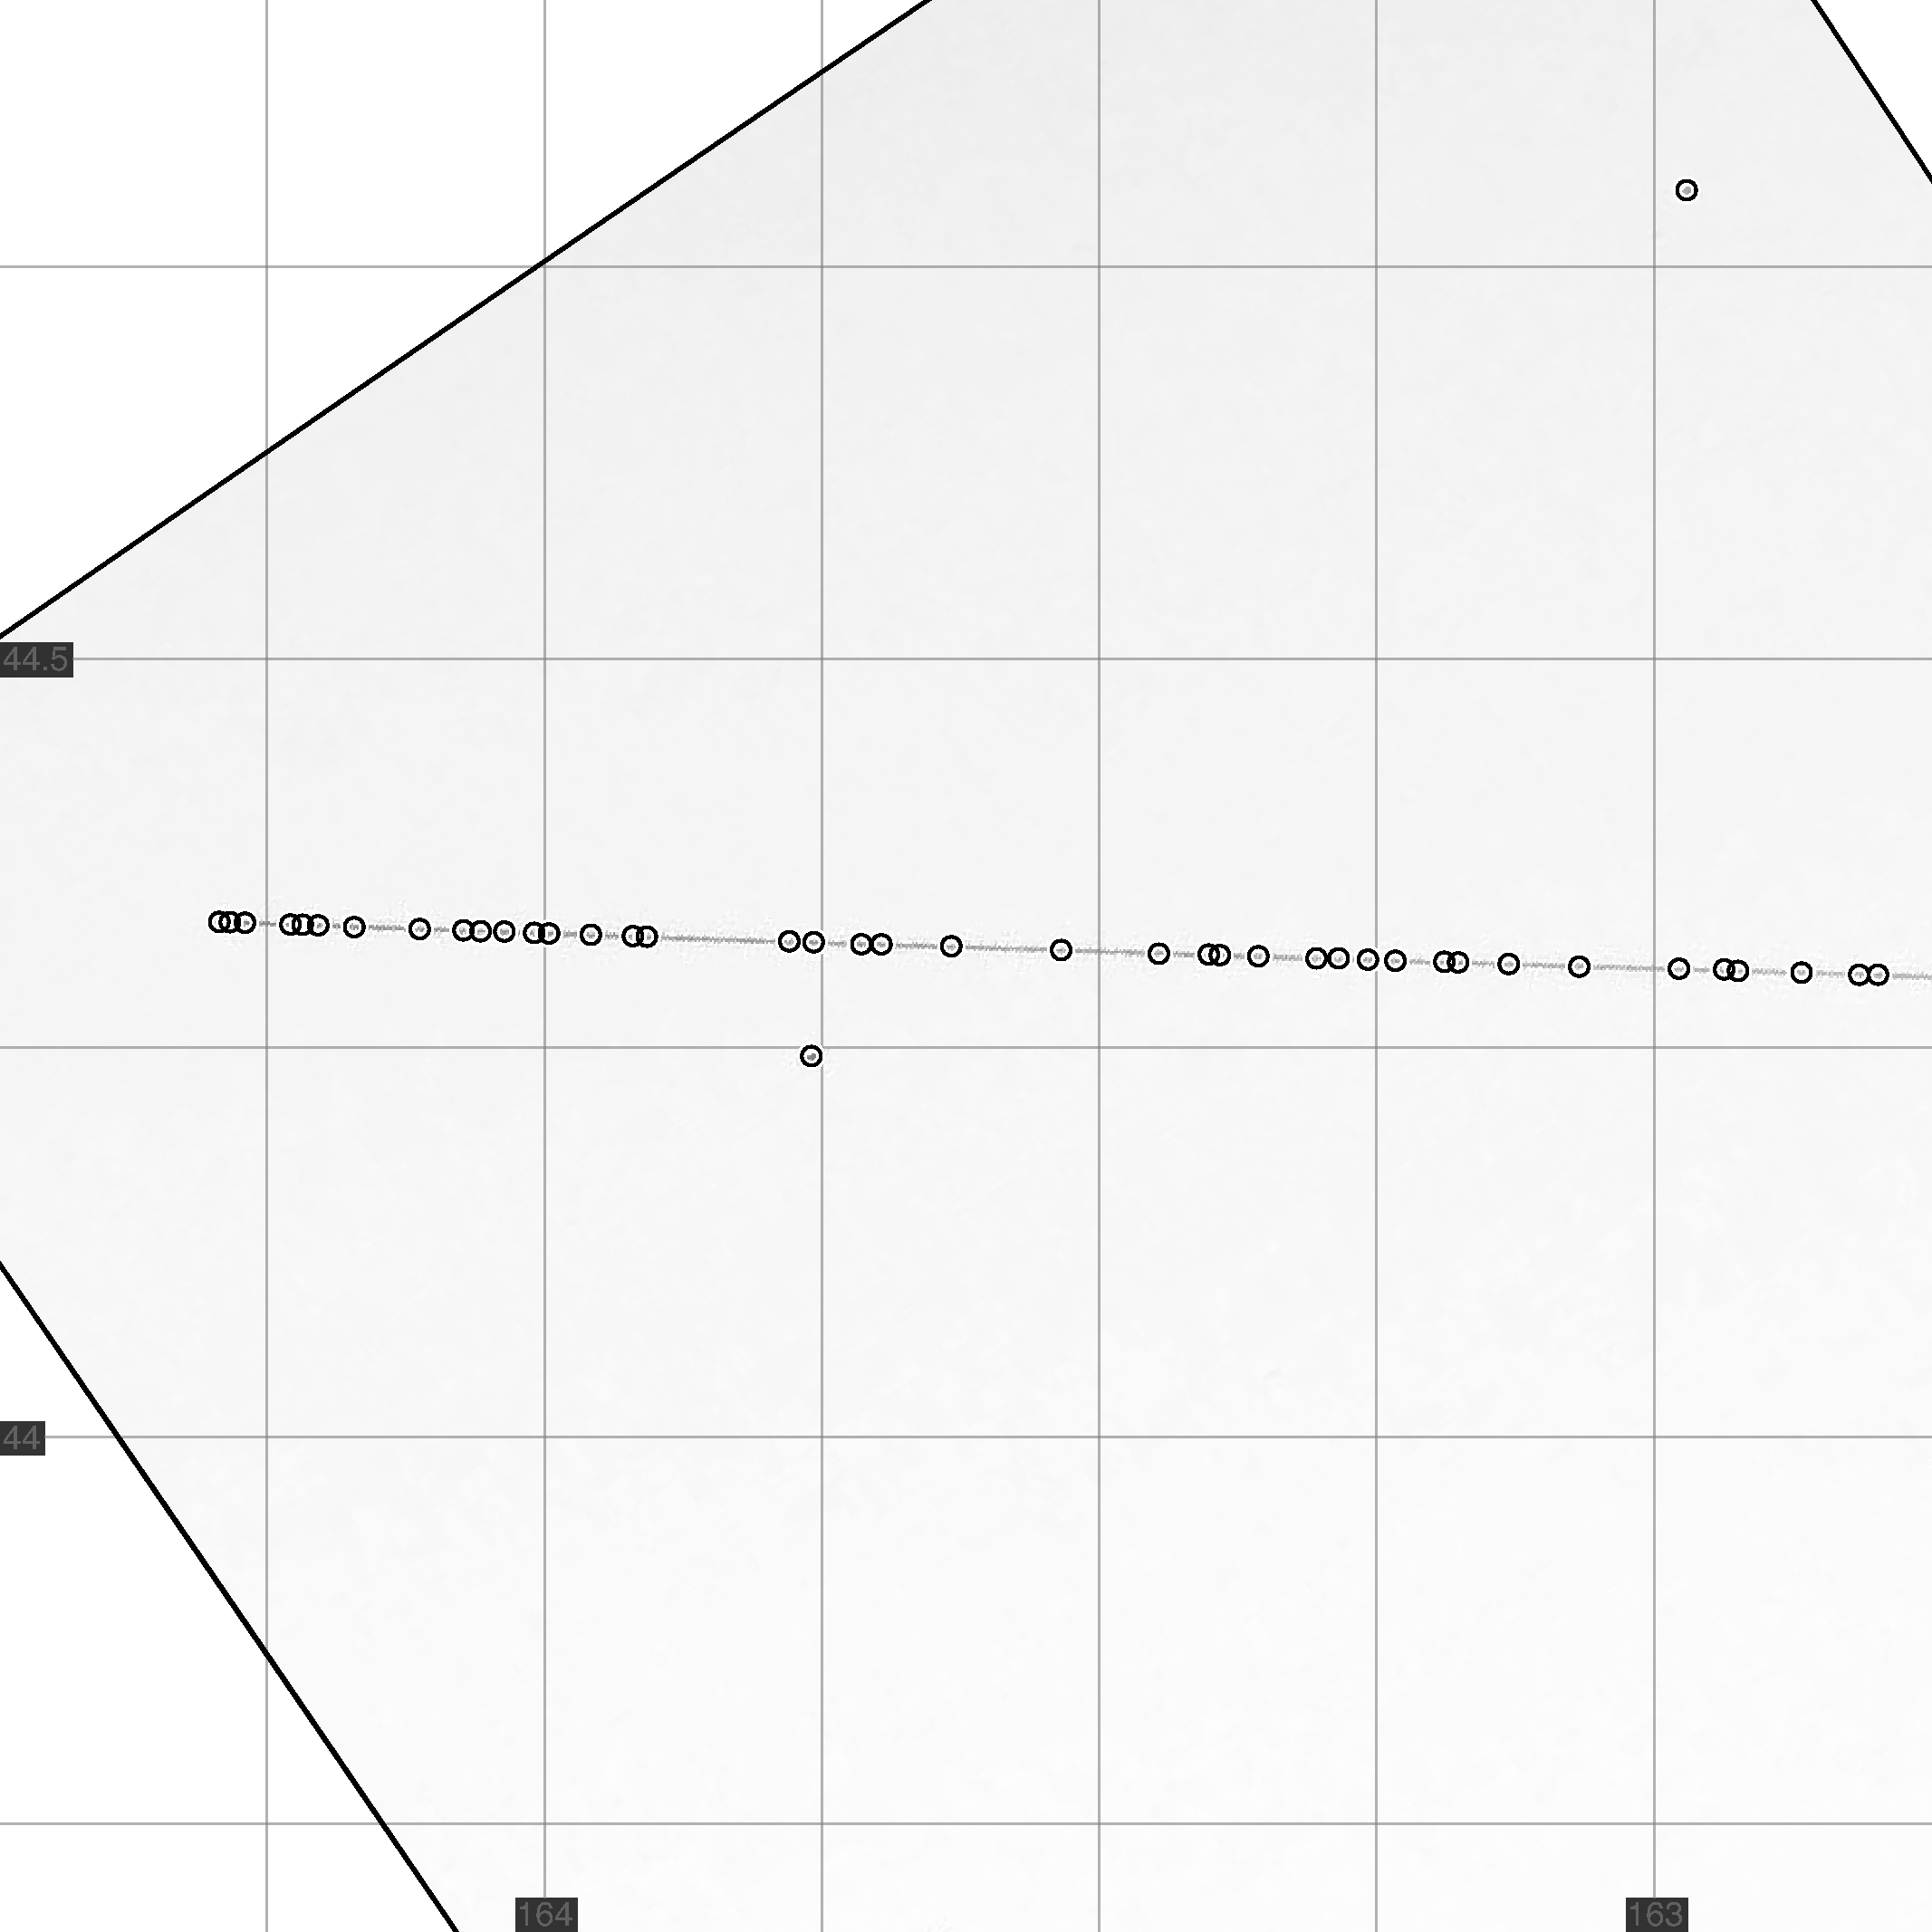
\includegraphics[width=0.55\textwidth]{iss-img-xy}}%
\\
\framebox{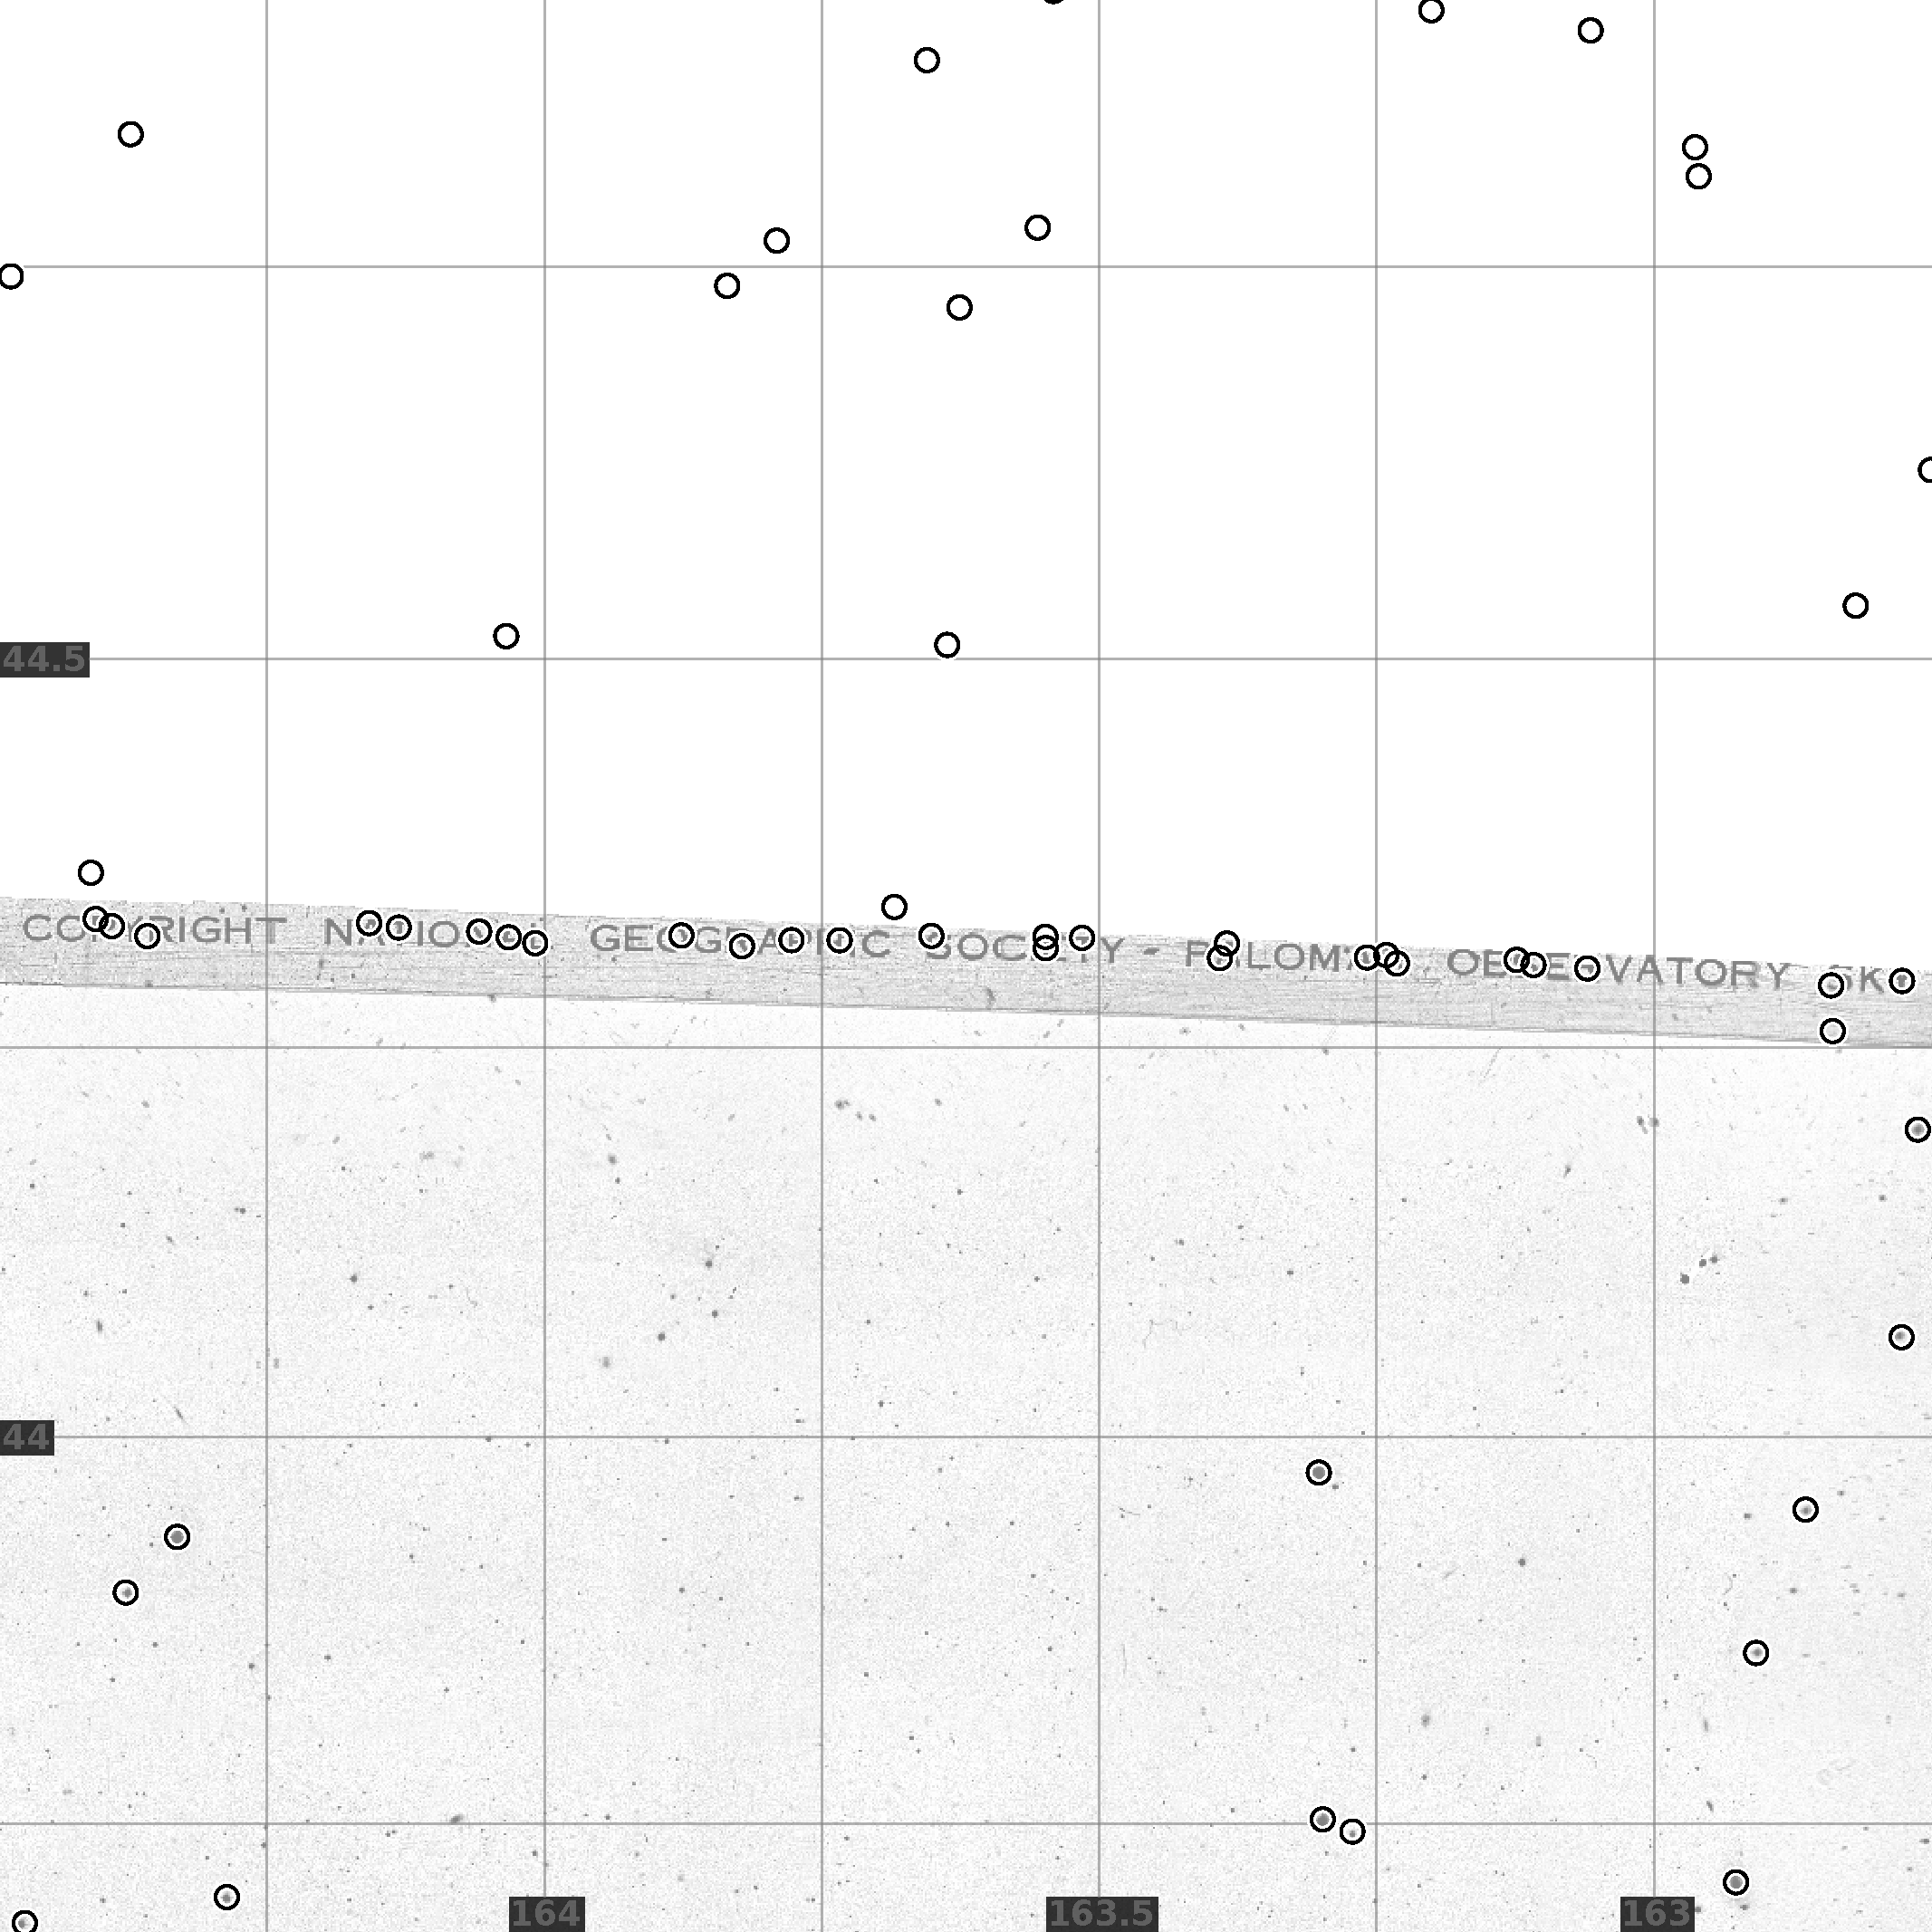
\includegraphics[width=0.55\textwidth]{iss-usnob-xy}}
\end{center}
\caption{A false-positive match (continued).  \captionpart{Top:} The
image, rotated to the alignment that our system found.  The circles
show the sources that were detected.  The linear feature becomes a
line of false sources.  \captionpart{Bottom:} The corresponding region
of the USNO-B plate.  The USNO-B source detection algorithm identifies
many false sources in the region of text.  The lines of sources in the
two images are aligned in this (false) match.
\label{fig:falseposB}}
\end{figure}


\end{document}
